%# -*- coding: utf-8-unix -*-
%%==================================================
%% chapter02.tex for SJTU Master Thesis
%% based on CASthesis
%% modified by wei.jianwen@gmail.com
%% Encoding: UTF-8
%%==================================================

\chapter{过程控制系统的错误序列注入攻击}
\label{chap:FSIattack}

\section{引言}
\label{sec:intro}

过程控制系统作为国家关键基础设施的基本组成部分已经广泛应用于工业和物联网系统中。正因为它们在现代工业社会中的关键作用,使得它们成为怀有恶意目的的攻击者的感染和侵袭的目标。传统的安全保护主要是通过多层网络防火墙和成熟的的病毒防御软件阻止网络攻击入侵工业网络。然而考虑到网络和复杂的硬件系统实施,这些方法不能完全保护网络和硬件平台免受不断变异的威胁侵入,例如Stuxnet病毒侵入人机界面(HMI)服务器并上传恶意代码到可编程逻辑控制器PLC使其损坏制造核原料的离心机。又因为HMI服务器通常是被安放在受良好保护的工业控制网络中,所以对其实施攻击是非常困难的。

本章我们提出的错误序列注入(FSI)攻击,可以通过感染和篡改PLC的输入信号迫使其执行误操作和破坏控制系统的关键设备。因为PLC的输入仅仅来自假设被FSI攻击注入的远程传感器,所以在不需要渗透到防御坚固的控制网络并执行恶意代码上传的情况下便可以对系统实施有目的性攻击。值得注意的是我们构造的攻击可以避开现有的系统故障检测机制,并利用其容错率漏洞来构造基于离散时间模型的FSI攻击。

\section{攻击模型概述}
\label{sec:formulation}

考虑到图\ref{fig1}描述的威胁模型,攻击者只需要侵入并控制遍布在远程的信号采集传感器。从过去的假数据注入攻击研究[5],[9],[19],[20],[30]中我们知道大部分工业控制系统包括电力系统的远程传感器如相量测量单元在实践中受到的保护较少并且分布在全国各地,因此与控制网络内的服务器相比更容易访问和侵入。我们假设攻击者知道高级基础设施配置,即连接到PLC传感器和执行器的输入输出的变量映射关系,这样攻击者不必渗透到控制网络中FSI攻击仍然可以成功。即使HMI服务器没有泄密而且攻击者也没有获得在PLC设备上上传恶意控制器程序的权限,我们构造的错误序列攻击只需要注入并控制向PLC发送测量信号的传感器便可以对控制系统造成不可逆的破坏。

\begin{figure}[!htb]
  \centering
  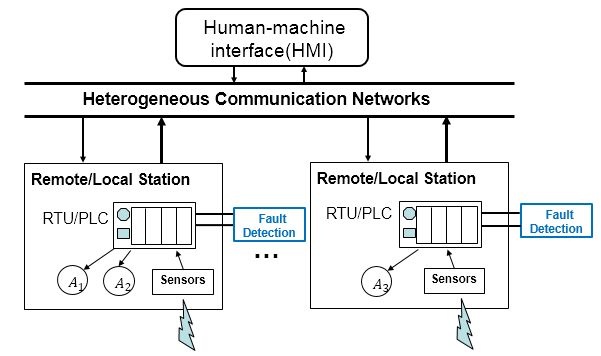
\includegraphics[scale=0.45]{att/threatModel1.png}
  \caption{FSI攻击威胁模型}
  \label{fig1}
\end{figure}

然而困难是如何在现有控制系统中部署成熟故障检测的情况下构建攻击使PLC执行误动作。FSI攻击的主要任务之一是分析并且绕开故障检测机制。通常来看用辨识精度不高的系统模型来检测随机性的故障能够得到很高的准确度,我们通过这一特性反向构造错误序列并且注入到受控制的远程传感器则可以达到使故障检测失效的目的。图\ref {fig2}显示了攻击是如何构造的。我们假设攻击者可以访问在PLC控制器和物理设备之间交换的信号或堆栈数据。然后利用输入和输出向量数据库,我们辨识出与故障检测的建模方法类似的无故障的离散事件模型。最后,我们搜索所有的不可被故障机制检测的虚假序列的集合,并且获得适当长度的恶意序列对受控制的传感器采集的输入信号进行篡改。

\begin{figure}[!htb]
  \centering
  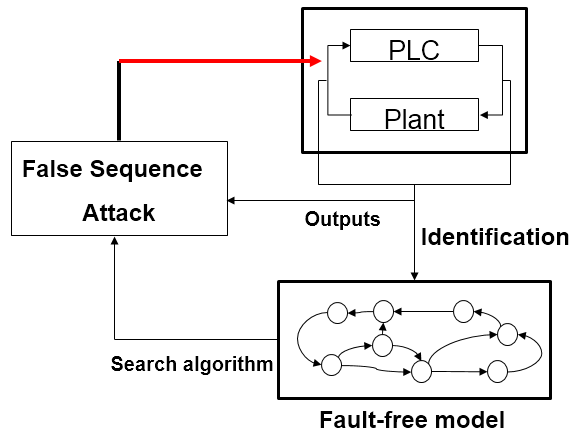
\includegraphics[scale=0.45]{att/ASC2.png}
  \caption{FSI攻击构造示意图}
  \label{fig2}
\end{figure}

\section{系统建模和攻击构造}
\label{sec:model}

我们需要一个形式化的描述来特征值为$m$的系统辨识模型$ \textbf{BEH}_{Ident}^m $和观测信号模型\( \textbf{BEH}_{Obs}^m \),从形式化模型定量生成特征值大于$m$特征向量。辨识的目标是使得在给定便是参数$k$的条件下特征值超出$k$的特征向量数目达到最小,理想情况是$ \textbf{BEH}_{Ident}^m $与$\textbf{BEH}_{Obs}^m $相等。最后我们在辨识得到的系统模型和观测信号模型基础上搜索FSI攻击序列。

\subsection{信号采集和观测特性定义}

我们通过在PLC控制器获取信号之后以固定时间间隔读取信号来采样数据\parencite {roth2012}。图\ref {fig3}显示了从PLC采样$I/O$向量序列的最常用的方法,通过OPC通信模式收集在服务端接收到的$I/O$数据形成标识数据库。

\begin{figure}[!htb]
  \centering
  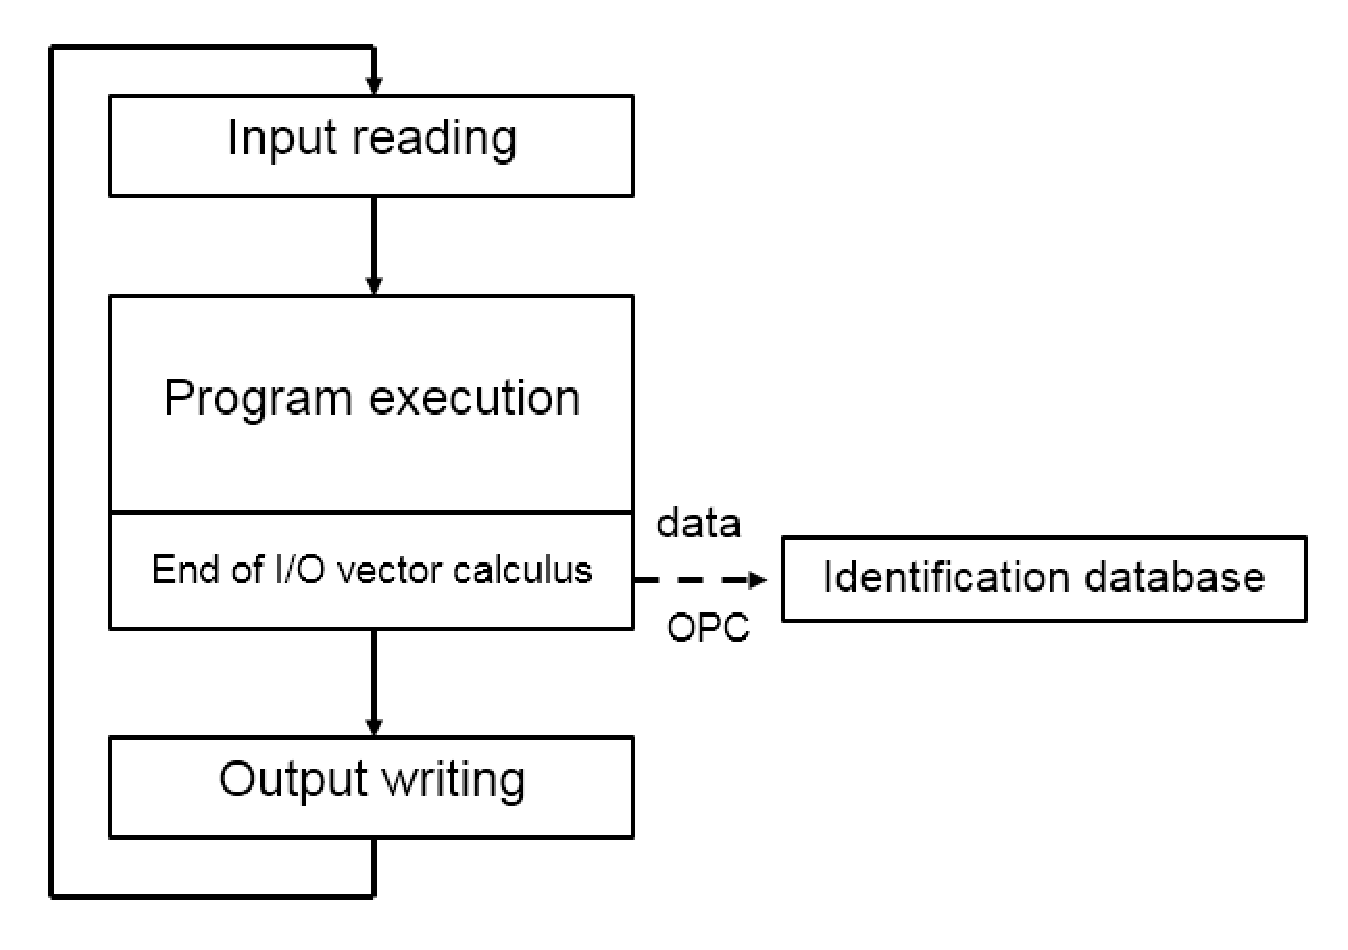
\includegraphics[scale=0.45]{att/database2.eps}
  \caption{对PLC采样数据示意图}
  \label{fig3}
\end{figure}

在实现数据收集之后,我们需要定义观察到的输入/输出($I/O$)序列、采样数据的语义和词义。 首先我们引入以下定义,

\textbf{定义1:} \( r \)个输入和$ s $ 个输出的采样数据的观测$I/O$序列集合定义为:

\begin{equation} 
\Sigma = (\gamma_1,...,\gamma_p) 
\end{equation} 这里 $\gamma_i = (u_i(1),u_i(2),...,u_i(|u_i|))$, $ u_i(j) $ 是向量$u$第$i$个分量的第$j$个输出,其中$ u = (I_1,...,I_r,O_1,\\...,O_s) = (IO_1,...IO_m) $ 且 $ m=r+s $。

我们假设对于$ \forall $两个连续的$I/O$向量$ u(t)\neq u(t + 1)$ 成立
当且仅当至少一个$I/O$向量分量改变且$I/O$向量是新生成的。

\textbf{定义2:} 观测到的采样数据词义集合表示和语义集合表示: 观测的词义可以用$I/O$序列长度为$q$的观测向量集合描述 
\[
L_{Obs}^q = \bigcup_{\gamma_i \in \Sigma} \Big(\bigcup_{t=1}^{|\gamma_i|-q+1} (u_i(t),u_i(t+1),...,u_i(t+q-1))\Big) 
\]

有了词义的形式化表示后,我们定义长度为$n$的采样数据的语义的表示:
\begin{equation}
 \textbf{BHE}_{Obs}^n = \bigcup_{i=1}^n L_{Obs}^i 
\end{equation}

\subsection{模型辨识}

\subsubsection{模型选择}

模型辨识的目的是确保辨识的任意长度为$ m $的语义表示$ \textbf {BEH}_{Ident}^m $等于观测到的任意长度为$ m $的语义表示  \( \textbf{BEH}_{Obs}^m \),其中$ m $可以是任何正整数。 简而言之,所辨识的模型在精度足够高的情况下能够完美复现基于PLC的过程控制系统。考虑到过程控制系统通常是可编程的控制器和物理设备的耦合系统,可编程的控制器可以被认为是确定性的,而物理设备通常被认为是非确定性的。因此,物理设备和控制器的耦合系统一定是非确定性的。因此,我们提出了适合于辨识过程控制系统的非确定性自发输出自动机(NDAAO)\parencite{klein2005}。

\textbf{定义3:} NDAAO是由5元组函数表示: \[ NDAAO=(X,\Omega,\textit{f}_{nd},\lambda,x_0) \] with\
\begin{itemize}
  \item $ X={x_0,...,x_{|x|-1}} $ 是有限状态集
  \item $ \Omega={\omega_1,...,\omega_{|\omega|}} $ 是有限输出变量集
  \item $ \textit{f}_{nd}: X\rightarrow 2^X $ 是非确定性转移函数
  \item $ \lambda: X\rightarrow \Omega $ 是状态对应的输出函数
  \item $x_0$ 是初始状态
\end{itemize}

NDAAO可以由图$G=(V,E)$的形式表示,图$G$的顶点集是NDAAO所有的状态集,有向边集是由非确定性转移函数$f_{nd}$组成,即\[ E(G)=\big\{(x_i,x_j)\in X\times X: x_j\in f_{nd}(x_i)\big\} \]每个节点对应一个状态并包含状态对应的输出,图~\ref{fig4}通过一个简单的例子来展示图形化的NDAAO模型。

\begin{figure}[!htb]
  \centering
  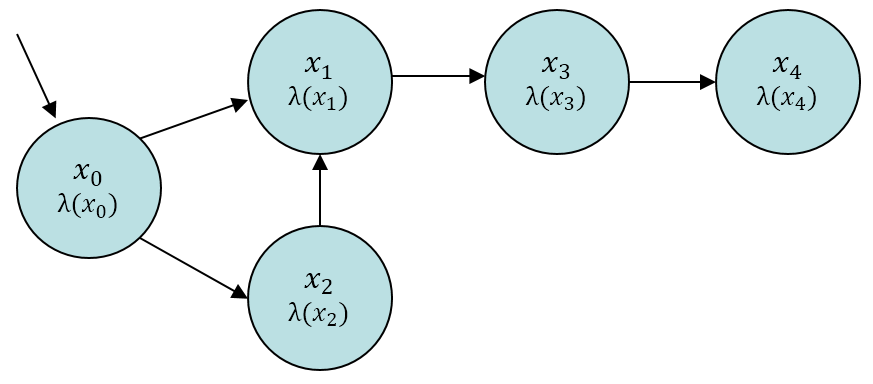
\includegraphics[scale=0.35]{att/ndaao_example.png}
  \caption{NDAAO图形表示}
  \label{fig4}
\end{figure}

\textbf{定义4:} NDAAO的词义和语义表示: 由初始状态为$x_i$的NDAAO生成的长度为$n$词语集合表示为
\begin{equation} 
W_{x_i}^{n}=\left\{\begin{split} &w\in \Omega^n~|~ w=\big( \lambda(x(1),...,\lambda(x(n))) \big):\\ 
&[\exists \big(x(1),...,x(n)\big): x(1)=x_i\in X,~and\\
&\forall\;1\leq t\leq n-1, x(t+1)\in f_{nd}(x(t))] \end{split} \right\} 
\end{equation} 然后由词语组成的长度为$n$词组集合表示
\begin{equation} 
W^n(NDAAO)=\bigcup_{x_i\in X} W_{x_i}^{n} 
\end{equation} 有了词组集合,我们可以获得NDAAO的长度为$n$语义集合表示
\begin{equation} 
\textbf{BEH}_{Ident}^n=\bigcup_{p=1}^n W^{p}(NDAAO) 
\end{equation}

\textbf{定义5:}辨识事件向量$\varepsilon(j)$是NDAAO中相邻两个辨识输出向量$\omega(j)$ 和 $\omega(j+1)$ 的变化量,用公式表示为 $\varepsilon=\omega(j+1)-\omega(j)$. 输入事件向量 $I(\varepsilon(j))$ 是相邻两个辨识输入向量 $I(j)$ 和 $I(j+1)$的变化量,同理输出事件向量$O(\varepsilon(j))$也有相似的定义. 具体的公式表示为:
\begin{equation} 
\varepsilon(j)=\bigcup_{l=1}^m \begin{cases}
I_l\_1~or~O_l\_1,~if~ I_l(j+1)-I_l(j)=1\\
I_l\_0~or~O_l\_0,~if~ I_l(j+1)-I_l(j)=-1\\
\epsilon,~if~ I_l(j+1)-I_l(j)=0
\end{cases} 
\end{equation}

考虑包含两个输入和一个输出的$I/O$向量序列$\gamma$,我们得到 \[\gamma=(A,B,C)=( \begin{bmatrix}
0\\1\\0
\end{bmatrix},\begin{bmatrix}
1\\1\\0
\end{bmatrix},\begin{bmatrix}
1\\0\\1
\end{bmatrix})\]

该序列可以简化表示成 $A\xrightarrow{I_1\_1}B\xrightarrow{I_2\_0,O_1\_1}C\cong A\xrightarrow{I_1\_1,I_2\_0,O_1\_1}C$

\subsubsection{辨识算法}

本节我们提出了一个辨识算法用来生成上一节中所描述的NDAAO模型。我们定义辨识参数$ k $用于确定用于生成新状态的$I/O$向量序列的长度。如果生成的NDAAO模型的长度为$ k $的语义集合正好与观测时采样数据产生的长度为$k$的语义集合一致的话,这样的NDAAO模型被称为$ k $完全可观测的。

NDAAO的构造主要分为三个步骤。首先,我们将观察到的序列转换为一组长度为$ k $的词组序列并在每组的第一个状态前创建一组长度为$ k-1 $ 伪状态以确保与其他词语一致。算法1的第一部分表示了观测序列的转换过程。然后我们开始执行NDAAO辨识操作, 将NDAAO的状态集与长度为$ k $的词组集相关联,并且转移函数由长度为$ k+1 $的词语表示。算法\ref{algo:ndaao}的第二部分表示了NDAAO的辨识过程​​。最后,我们合并等效状态来对状态空间进行降维,对于任意两个不同的状态$ x_i $和$ x_j $,如果它们相关联的输出相同并且它们具有相同的后继状态集,则我们可以将这两个状态合并到一个状态。我们通过从NDAAO的状态集和转移函数绘制状态转移图来使模型可视化。具体过程如算法\ref{algo:graph}所示。

\begin{algorithm}[h]
  \caption{NDAAO构造算法}
  \label{algo:ndaao}
  \begin{algorithmic}[1]
    \Require %算法的输入参数:Input
    观测的$I/O$序列(采样数据) $\varSigma$ 和辨识参数 $k$
    \Ensure %算法的输出:Output
    NDAAO模型和状态转移图 $G=(V,E)$;  \\
    // \textbf{第一部分:观测序列的转换过程}
    \For{each $\gamma_i \in \varSigma$}
      \If {$u_i(1)\neq u_i(|\gamma_i|)$}
          \State  从$\varSigma$删除$\gamma_i$; Return;\
        \Else
        \State $\alpha_i(t)=\begin{cases}
        u_i(1),\quad for ~~ 1\leq t\leq k-1\\
        u_i(t-k+1),\quad for ~~ k \leq t \leq k+|\gamma_i|-1
        \end{cases}$\
        \For {$m=1~~to~~|\gamma_i|$}
        \State $w_i(m)=(\alpha_i(m),...,\alpha_i(m+k-1))$;
        \EndFor
        \State $\gamma_i^k=(w_i(1),...,w_i(|\gamma_i|))$;
        \EndIf
    \EndFor
    \State $\varSigma^k=\bigcup\limits_{i=1}^{|\varSigma|}  \gamma_i^k$;\\
    \State \textbf{第二部分:NDAAO的辨识过程​​}初始化状态集 $X=\emptyset$, 转移函数 $f_{nd}(x_0)=\emptyset$, 输出 $\Omega=\emptyset$, 初值状态 $x_0=\varSigma^k[0][0]$, 节点集 $N=\emptyset$ 和边集 $E=\emptyset$;
    \ForAll {$\xi$ such that $\xi \in \varSigma^k$} 
      \ForAll {$\eta$ such that $\eta \in \xi$}
      \State $X\leftarrow X\cup \xi$; $\Omega \leftarrow\ \Omega \cup \eta(|\eta|)$;
      \EndFor
    \EndFor
    \ForAll {$\delta$ such that $\delta \in \varSigma^{k+1}$} 
      \ForAll {$\psi$ such that $\psi \in \delta$}
      \State $x \leftarrow \psi[1-k]$;$f_{nd}(x)=\psi[k-|\psi|]$;  
      \EndFor
    \EndFor
  \end{algorithmic}
\end{algorithm}

\begin{algorithm}[h]
  \caption{状态空间降维和图形化表示}
  \label{algo:graph}
   \begin{algorithmic}[1]
\ForAll {$x_i,x_j$ such that $x_i,x_j \in X and i\neq j$}
      \If {$\lambda(x_i)=\lambda(x_j)$ 和 $f_{nd}(x_i)=f_{nd}(x_j)$}
        \State 合并 $x_i$ 和 $x_j$, 从$X$中删除 $x_i(x_j)$ 并且用$f_{nd}(x_{pre})=x_j(x_i)$替换$f_{nd}(x)=x_i(x_j)$, 这里$x_{pre}$是$x_i(x_j)$的前继;  
      \EndIf
    \EndFor
    \State $V\leftarrow\ V\cup X$;
    \State $E \leftarrow E\cup (x,f_{nd}(x))$;
    \State 对$G(V,E)$画图;
  \end{algorithmic}
\end{algorithm}
\textbf{例子1.} 考虑从无故障例子系统中采样三组向量序列: $\gamma_1=(A,B,C,D,E,A)$, $\gamma_2=(A,B,D,C,\\D,E,A)$, $\gamma_3=(A,D,B,C,D,F,E,A)$。 大写字母代表不同的$I/O$向量。这里我们选取辨识参数$k=2$,经过序列转换后我们得到 \[\begin{split} \gamma_1^{k=2}&=(AA,AB,BC,CD,DE,EA)\\ \gamma_2^{k=2}&=(AA,AB,BD,DC,CD,DE,EA)\\\gamma_3^{k=2}&=(AA,AD,DB,BC,CD,DF,FE,EA) \end{split}\] 和 \[\begin{split} \gamma_1^{k=3}&=(AAA,AAB,ABC,BCD,CDE,DEA)\\ \gamma_2^{k=3}&=(AAA,AAB,ABD,BDC,DCD,CDE,DEA)\\\gamma_3^{k=3}&=(AAA,AAD,ADB,DBC,BCD,CDF,\\&\quad \ DFE,FEA) \end{split}\]

在获得$\Sigma^{k=2}$ 和 $\Sigma^{k=3}$之后,我们从$\Sigma^{k=2}$得到状态集并且通过算法\ref{algo:ndaao}的第二部分从$\Sigma^{k=3}$得到转移函数。相应的例子示意如图~\ref{fig5}所示。

\begin{figure}[!htb]
  \centering
  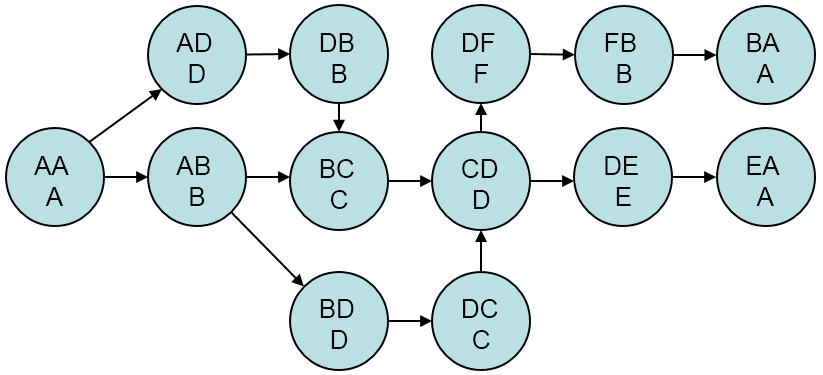
\includegraphics[scale=0.40]{att/2dot_graph.png}
  \caption{经过两步辨识算法得到的NDAAAO模型图示}
  \label{fig5}
\end{figure}

初始辨识的模型相比真实系统存在冗余的状态集和边集,因此需要根据算法\ref{algo:ndaao}的第三部分来减少状态空间以简化初始模型。在例1中如果我们将状态$ DB $与状态$ AB $、状态$ BA $与状态$ EA $、状态$ BC $与状态$ DC $均合并,并且对任意$x_i \in X$用$x_i$替换长度为$k$的向量词语。我们得到的简化NDAAO模型如图~\ref{fig6}所示。

\begin{figure}[!htb]{}
  \centering
  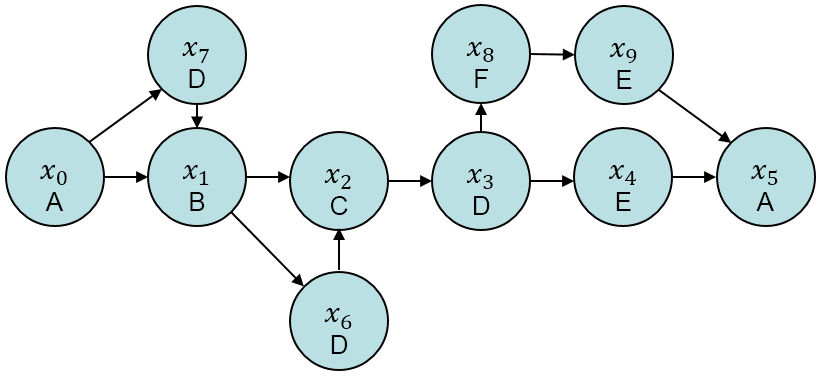
\includegraphics[scale=0.40]{att/3dot_graph.png}
  \caption{最终简化的NDAAO模型图示}
  \label{fig6}
\end{figure}

\subsection{FSI攻击的构造}

在我们辨识出无故障的NDAAO之后,我们可以利用故障检测的原理构造不可检测的错误序列。我们知道,故障检测是根据当前观测的$I/O$向量与辨识的NDAAO的预期输出是否一致来确定是否存在故障的。如果结果为真,则认为当前观测向量安全,否则给出警报可能存在故障。在我们的攻击方法中,我们构造了错误序列注入攻击,其不仅满足序列输出来自辨识的模型以确保不能被故障机制检测到,而且还通过选择具有恶意执行逻辑的适当长度的错误序列注入到控制器的输入信号中来破坏系统。从$ x_i $开始的长度为$ n $的错误序列的具体形式描述如下定义,
\begin{equation} 
S_{x_i}^{n}=\left\{\begin{split} &s\in \Omega^n~|~s=\big( \lambda(x(1),...,\lambda(x(n))) \big)\wedge\\
&(s\notin L_{Obs}^n):[\exists \big(x(1),...,x(n)\big): x(1)\\&=x_i\in X,~and~
\forall\;1\leq t\leq n-1,\\&x(t+1)\in f_{nd}(x(t))] \end{split} \right\} 
\end{equation}

上述定义的$ S_{x_i}^{n} $从辨识的NDAAO模型中截取长度为$ n $的序列并且不同于观测到的$I/O$向量集的任何长度为$ n $的序列。因此,定义的错误序列当注入到控制器的输入信号时能够对控制系统造成潜在的入侵破坏。由于降维的NDAAO是$(k + 1)$完全可观测,故以下等式成立:
\begin{equation} 
\forall~m\leq k+1,~~\textbf{BEH}_{Obs}^m=\textbf{BEH}_{Ident}^m 
\end{equation}

根据上述理论,只有当$ S_ {x_i} ^ {n} $中长度不小于$ k-2 $的序列才可以是错误序列。我们基于辨识参数$ k $ 获得从NDAAO生成的所有错误序列集合为
\begin{equation} 
A^k=\bigcup_{x_i\in X} \big( \bigcup_{n=k+2}^{max(|\gamma_d|)} (S_{x_i}^{n})\big),~\gamma_d\in \Sigma \end{equation}

在我们得到错误序列的定义之后,下一步是提出搜索算法以获得所有不可被故障机制检测的错误序列集合。从算法\ref{algo:fsi}可以看出使用FSI递归遍历算法的递归公式可以获得长度不小于$ k + 2 $的错误序列,这些序列来自于NDAAO模型选择且不存在于开始状态为$ x_ {init} $的观测$I/O$向量的序列的任意子序列。通过获取FSI递归遍历算法的输出,我们合并所有$ X $中始于状态$ x_ {init} $的$ S_ {x_ {init}} $的序列集合$ A ^ k $,具体表达式如下,
\begin{equation} 
A^k=\bigcup_{x_{init}\in X} \big(S_{x_{init}}\big) 
\end{equation}


\begin{algorithm}[h]
  \caption{FSI递归遍历算法}
  \label{algo:fsi}
  \begin{algorithmic}[1]
    \Require %算法的输入参数:Input  
    辨识的NDAAO模型, 观测的$I/O$序列 $\varSigma$, 辨识参数 $k$ 和初始状态 $x_{init}$ \\  
    
    \Ensure %算法的输出:Output  
    错误序列集合 $S_{x_{init}}$;  \\
    \For{each $x \in x_{init}$}
      \State $x_{init}=f_{nd}(x)$
      \State $seq$.append$(x)$
      \State $IncSearching(NDAAO,\varSigma,k,x_{init})$
      \If {$|seq|\geq (k+2)$ and $ seq\notin substring(\gamma) ~for~\forall\gamma\in\varSigma$}
        \State $S_{x_{init}}$.append$(seq)$
      \EndIf
      \State $seq$.pop()
    \EndFor
    \State Return $S_{x_{init}}$
  \end{algorithmic}
\end{algorithm}

通过算法\ref{algo:fsi},获得的示例1的错误序列的集合是\[{(A,D,B,D,...),(...,D,C,D,F,...),(A,B,C,D,F,...)}\]其中字母之前或之后的省略号可以是字母的任何前导或后继。

因为攻击者可能对来自控制系统的传感器的控制有限,我们需要确定在从上述方法产生的错误序列的两个连续向量之间变化的$I/O$向量分量。

\subsection{可行性和性能指标}

本文攻击的可行性主要来自两方面。 首先随着辨识参数$ k $的增加,NDAAO的状态空间迅速增加并且需要采样庞大的顺序系统进程周期信号数据才能使模型收敛到稳定水平\parencite{klein2005}。因此,当在精度值$ k $较大的条件下进行在线检测时往往需要大量的计算。 我们的工作主要实现离线攻击,有足够的时间进行计算。其次,考虑到检测机制的稳定性和性能,在实际工业系统中通常一个较小的参数$ k $足以满足基于故障检测的实际要求\parencite{roth2012},也正是因为这两个条件,较小的参数$ k $能够为我们的攻击的构造提供良好的可行性。

为了评估NDAAO的连通性,我们给出由一个状态产生的后继边的平均数量的信息。 我们定义结构复杂度指标$ C_s $ 如下:
\begin{equation}
C_s= \dfrac{\sum_{x_i\in X} (deg(x_i))}{|X|} 
\end{equation} 这里 $deg(x_i)=|f_{nd}(x_i)|$ 是状态$x_i$的度.

与复杂性指标类似,我们定义攻击脆弱度指数来衡量从已辨识的NDAAO模型中搜索错误序列的成功率。攻击脆弱度指数定义如下所示:
\begin{equation}
 C_A^n=\dfrac{|\bigcup_{x_i \in X}(A_{x_i}^n)|}{|W_{Ident}^n|} 
 \end{equation}

通过方程(11)和(12),我们可以获得所有状态的多重分支状态的比率和所有辨识的$I/O$序列集中错误序列的比率。
\section{实验仿真}
\label{sec:simulation}

为了证明所提出的错误序列攻击方法的可行性和性能,我们给出了相应的案例仿真。 考虑的系统是一个小型的货物分拣系统,该系统的功能是根据尺寸大小分拣包裹。系统有11个输入(来自物理设备的输出信号)和5个输出(从PLC输入到物理设备的信号)。 图\ref{fig7}显示了货物分拣系统的结构示图。
\begin{figure}[!htb]
  \centering
  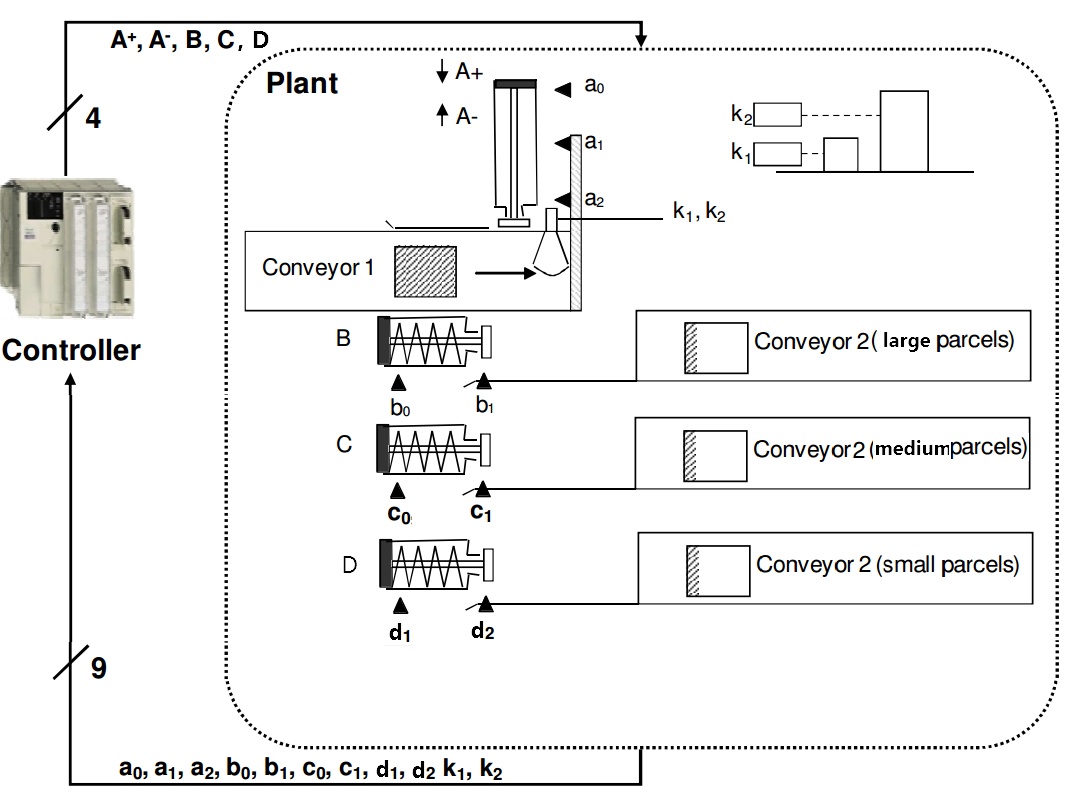
\includegraphics[scale=0.38]{att/sort.png}
  \caption{货物分拣系统的结构示图}
  \label{fig7}
\end{figure}

\begin{figure}[!htb]
  \centering
  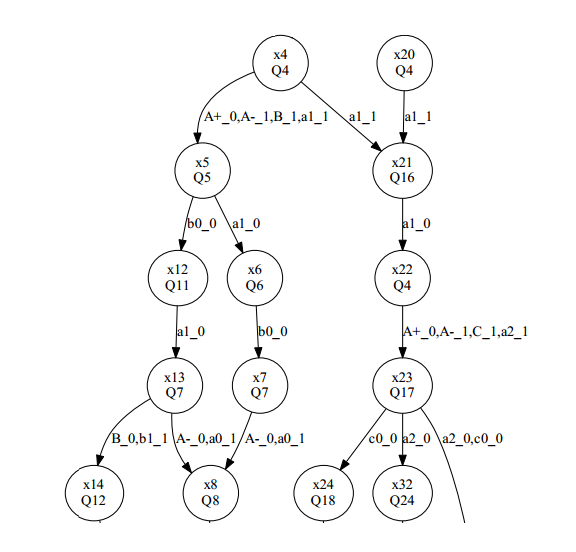
\includegraphics[scale=0.46]{att/casendaao.png}
  \caption{货物分拣系统的部分NDAAO模型}
  \label{fig8}
\end{figure}


辨识数据库是由50个采样的系统运行周期组成并且每个周期的采样时间均为货物到来和分拣时刻。系统的输入和输出变量向量为$[A+,A-,B,C,D,k_1,k_2,a_0,a_1,a_2,b_0,b_1,c_0,c_1,d_0,d_1]$。在完成辨识过程和状态空间降维后,我们得到货物分拣系统完整的NDAAO模型,由于篇幅所限部分模型如图\ref{fig8}所示。
\begin{figure}[!htb]
  \centering
  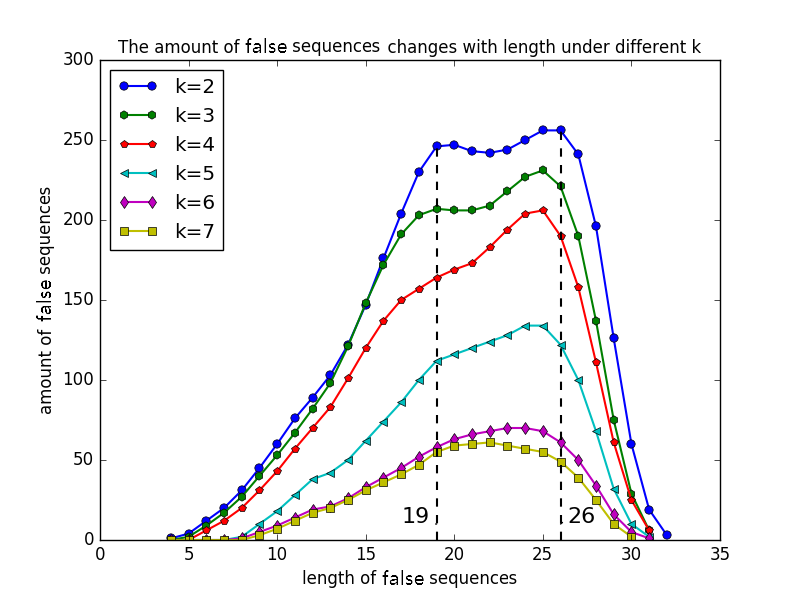
\includegraphics[scale=0.42]{att/length.png}
  \caption{不同数量的错误序列数量}
  \label{fig9}
\end{figure}

\begin{figure}[!htb]
  \centering
  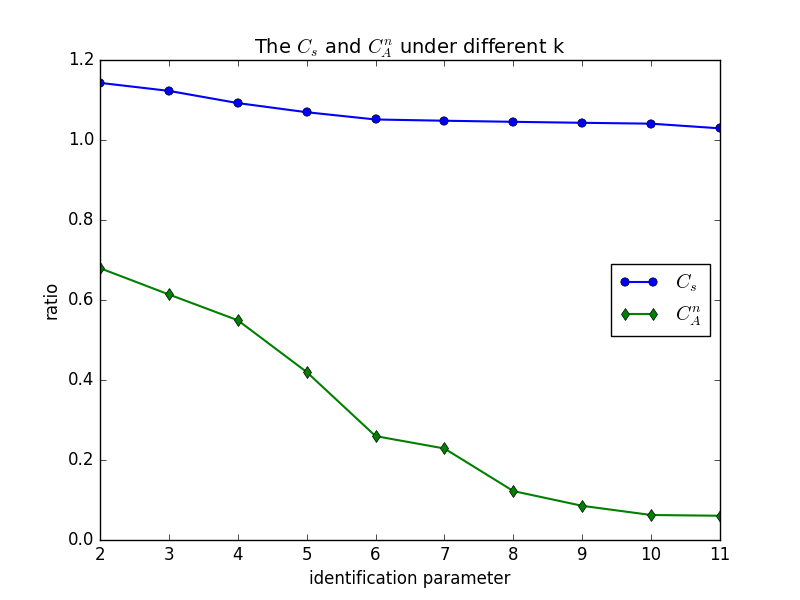
\includegraphics[scale=0.46]{att/vuln.png}
  \caption{$C_s$ 的 $C_A^n$关系}
  \label{fig10}
\end{figure}

通过获得的模型,我们执行了错误序列搜索过程,在简化之前我们搜索了大量不同长度的假序列,这些错误序列可以作为潜在的恶意逻辑顺序注入到受控传感器中。例如\[\begin{split} A_1&=Q_{34}Q_{21}Q_{22}Q_{30}\\A_2&=Q_{32}Q_{10}Q_{11}Q_{12}Q_{28}\\A_3&=Q_{16}Q_{17}Q_{18}Q_{19}Q_{20}Q_{34} \end{split}\]这里$Q_i$是每个观测周期的输出向量。\\

然而如果攻击者实施攻击,必须需要保证上述序列所有的传感器受到感染和控制,这在实际操作中是很难实现的。因此我们需要使用来自等式(6)的驱动事件向量简化处理如上所述在序列集,结果如下:\[\begin{split} A_1&=Q_{34}\xrightarrow{d1\_1,b0\_1,\{b0\_0,d0\_1\}}Q_{30}\\A_2&=Q_{32}\xrightarrow{d1\_1,b1\_1,k2\_1,\{b1\_0,d0\_1\}}Q_{28}\\A_3&=Q_{16}\xrightarrow{\{k1\_0,a0\_0,c1\_1d1\_0\},a1\_1,a1\_0,k2\_1,\{a2\_1,c1\_0\}}Q_{34} \end{split}\]这里,用逗号分隔的每个箭头的符号序列是在错误序列的每两个向量之间的单个驱动事件输入的集合。当我们注入这些错误序列到PLC控制器的输入信号时,在没有被故障机制所检测的情况下,分拣结束后将获得错误的分拣结果。
从获得的假序列,我们发现大多数假序列集中在19和26之间的长度。所以潜在的恶意攻击可以选择这种长度的假序列。图。\ref{fig9}显示了不同$ k $下假序列变化的长度。
考虑到良好的攻击可行性需要较大的状态度和较多的多分支状态,图\ref{fig10}显示了在结构复杂度度量$ C_s $(多分支状态的比率)减小的情况下,攻击脆弱度指数(错误序列的占比)快速下降。因此我们可以通过在多个分支状态上添加特定的检测机制来避免这种攻击,而不是一味地提高辨识参数$ k $。

\section{本章小结}

在本章中,我们基于过程控制系统提出了一种错误序列注入攻击,所获得的错误序列攻击将被用作注入到与PLC连接的远程传感器接收的信号来对系统进行恶意逻辑攻击。我们给出了包括FSI递归搜索算法在内的错误序列注入攻击构建的整个实现过程。值得注意的是对多个分支状态的检测将成为对这种攻击的有效防御。实验仿真表明我们的方法是对部署故障检测的控制系统造成一定的破坏性威胁并证明我们提出的方法的有效性。

\label{sec:insertimage}

